% handout
\documentclass[11pt,final,usepdftitle=false]{beamer}
\mode<presentation>
\usetheme{ln12en}
\graphicspath{{\logopath}{\picspath}{\figspath}{./logos/}{./pics/}{./figs/}}
\usepackage{listings}
%\usepackage{bera}
\usepackage{inconsolata}
\usepackage{moresize}
\usepackage{ucs}
\usepackage{framed}
\usepackage{adjustbox}
%\renewcommand*\ttdefault{cmvtt}


\hypersetup{pdftitle={Lucas Nussbaum - systemd}}
\title{systemd}
\authorteaching
\instituteiutlp
\newcommand{\tilda}{\textasciitilde{}}
\date{}


% \AtBeginSection[]
% {
%   \begin{frame}
%     \frametitle{Outline}
%     \tableofcontents[currentsection]
%   \end{frame}
% }

\usepackage{tikz}
\usetikzlibrary{shapes,arrows,positioning}
\newcommand{\Gentsroom}{{\fontfamily{mvs}\fontencoding{U}\fontseries{m}\fontshape{n}\selectfont\char120}}

\begin{document}

\frame{\titlepage}

\begin{frame}{Outline}
	\tableofcontents
\end{frame}

\section{Introduction}

\begin{frame}{Init system}
\begin{itemize}
\item First process started by the kernel (pid 1)
	\hbr
\item Responsible for bringing up the rest of userspace
	\begin{itemize}
		\item Mounting filesystems
		\item Starting services
		\item \ldots
	\end{itemize}
	\hbr
\item Also the parent for orphan processes
	\hbr
\item Traditional init system on Linux: sysVinit
	\begin{itemize}
		\item Inherited from Unix System V
		\item With additional tools (insserv, startpar) to handle dependencies and parallel initialization
	\end{itemize}
\end{itemize}
\end{frame}

\begin{frame}{systemd}
	\begin{itemize}
		\item Written (since 2010) by Lennart Poettering (Red Hat) and others
			\hbr
		\item Now the default on most Linux distributions
			\hbr
		\item Shifts the scope from \textsl{starting all services} (sysVinit) to\\
			\alert{managing the system and all services}
			\hbr
		\item Key features:
			\begin{itemize}
				\item Relies on cgroups for
					\begin{itemize}
						\item Services supervision
						\item Control of services execution environment
					\end{itemize}
					\hbr
				\item Declarative syntax for unit files $\leadsto$ more efficient/robust
					\hbr
				\item Socket activation (on-demand startup of services)
					\hbr
				\item Nicer user interface (systemctl \& friends)
			\end{itemize}
			\hbr
		\item Additional features: logging, timer units (cron-like), user sessions handling, containers management
	\end{itemize}
\end{frame}

\section{Behind the scenes: cgroups}

\begin{frame}{Behind the scenes: cgroups}
\begin{itemize}
\item Abbreviated from \textsl{control groups}
\hbr
\item Linux kernel feature
\hbr
\item Limit, account for and isolate \alert{processes and their resource usage} (CPU, memory, disk I/O, network, etc.)
\hbr
\item Related to \textsl{namespace isolation}:
	\begin{itemize}
		\item Isolate processes from the rest of the system
			\hbr
		\item \textsl{Chroots on steroids}
			\hbr
		\item PID, network, UTS, mount, user, etc.
	\end{itemize}
			\hbr
		\item LXC, Docker $\approx$ cgroups + namespaces (+ management tools)
\end{itemize}
\end{frame}

\begin{frame}{cgroups and systemd}
	\begin{itemize}
	\item Each service runs in its own cgroup
		\hhbr
	\item Enables:
		\begin{itemize}
			\item Tracking and killing all processes created by each service
				\hhbr
			\item Per-service accounting and resources allocation/limitation
		\end{itemize}
		\hhbr
	\item Previously, with sysVinit:
		\begin{itemize}
			\item No tracking of which service started which processes
				\begin{itemize}
					\item PID files, or hacks in init scripts: \texttt{pidof} / \texttt{killall} / \texttt{pgrep}
						\hhbr
					\item Hard to completely terminate a service (left-over CGI scripts when killing Apache)
				\end{itemize}
				\hbr
			\item No resources limitation (or using \texttt{setrlimit} (= \texttt{ulimit}), which is per-process, not per-service)
		\end{itemize}
	\hhbr
	\item Also isolate user sessions $\leadsto$ kill all user processes (not by default)
	\hhbr
\item More information: \href{http://0pointer.net/blog/projects/cgroups-vs-cgroups.html}{\ul{Control Groups vs. Control Groups}} and\\ \href{http://0pointer.net/blog/projects/systemd-for-admins-2.html}{\ul{Which Service Owns Which Processes?}}
\end{itemize}
\end{frame}



\begin{frame}{\texttt{systemd-cgls}: visualizing cgroup hierarchy}
% export GTK_MODULES=/usr/lib/gtk-3.0/modules/libgtk-vector-screenshot.so
% take-vector-screenshot
\hbr

\includegraphics[height=0.9\textheight]{figs/systemd-cgls}
\end{frame}

\begin{frame}{\texttt{systemd-cgtop}: per-service resources usage}
\begin{framed}

\includegraphics[width=1\textwidth]{figs/systemd-cgtop}
\end{framed}
Note: requires enabling \texttt{CPUAccounting}, \texttt{BlockIOAccounting}, \texttt{MemoryAccounting}
\end{frame}

\section{Managing services}

\begin{frame}{Managing services with \texttt{systemctl}}
	\begin{itemize}
		\item What is being manipulated is called a  \textsl{unit}: services (.service), mount points (.mount), devices (.device), sockets (.socket), etc.
			\hbr
		\item Basic commands:
\hbr
	\end{itemize}
	\resizebox{\textwidth}{!}{
	\begin{tabular}{|c|c|c|}
		\hline
		sysVinit & systemd & notes \\
		\hline
		service foo start & systemctl start foo & \\
		service foo stop & systemctl stop foo & \\
		service foo restart & systemctl restart foo & \\
		service foo reload & systemctl reload foo & \\
		service foo condrestart & systemctl condrestart foo & restart if already running \\
		update-rc.d foo enable & systemctl enable foo & auto-start at next boot \\
		update-rc.d foo disable & systemctl disable foo & disable auto-start \\
		& systemctl is-enabled foo & \\
		\hline
	\end{tabular}}
	\begin{itemize}
		\item There's auto-completion (\texttt{apache2} and \texttt{apache2.service} work)
		\hbr
		\item Several services can be specified:\\
			\texttt{systemctl restart apache2 postgresql}
		\hbr
	\end{itemize}
\end{frame}

\begin{frame}{systemd and runlevels}
	\begin{itemize}
		\item With sysVinit, runlevels control which services are started automatically
			\begin{itemize}
				\item 0 = halt; 1 = single-user / minimal mode; 6 = reboot
				\item Debian: no difference between levels 2, 3, 4, 5 (multi-user)
				\item RHEL: 3 = multi-user text, 5 = multi-user graphical
			\end{itemize}
			\hbr
		\item systemd replaces runlevels with \alert{targets}:
			\begin{itemize}
				\item Configured using symlinks farm in \texttt{/etc/systemd/system/\textbf{target}.wants/}
					\hbr
				\item \texttt{systemctl enable}/\texttt{disable} manipule those symlinks
					\hbr
				\item \texttt{systemctl mask} disables the service and prevents it from being started manually
					\hbr
				\item The default target can be configured with\\ \texttt{systemctl get-default/set-default}
					\hbr
				\item More information: \href{http://0pointer.net/blog/projects/three-levels-of-off.html}{\ul{The Three Levels of "Off"}}
			\end{itemize}
	\end{itemize}
\end{frame}

\begin{frame}[fragile]{Default targets (\texttt{bootup(7)})}
\begin{center}
\begin{adjustbox}{height=0.45\textheight,keepaspectratio}
\begin{lstlisting}[basicstyle=\ttfamily\tiny,escapeinside={<<}]
local-fs-pre.target
         |
         v
(various mounts and   (various swap   (various cryptsetup
 fsck services...)     devices...)        devices...)       (various low-level   (various low-level
         |                  |                  |             services: udevd,     API VFS mounts:
         v                  v                  v             tmpfiles, random     mqueue, configfs,
  local-fs.target      swap.target     cryptsetup.target    seed, sysctl, ...)      debugfs, ...)
         |                  |                  |                    |                    |
         \__________________|_________________ | ___________________|____________________/
                                              \|/
                                               v
                                        sysinit.target
                                               |
          ____________________________________/|\________________________________________
         /                  |                  |                    |                    \
         |                  |                  |                    |                    |
         v                  v                  |                    v                    v
     (various           (various               |                (various          rescue.service
    timers...)          paths...)              |               sockets...)               |
         |                  |                  |                    |                    v
         v                  v                  |                    v               <\textbf{rescue.target}<
   timers.target      paths.target             |             sockets.target
         |                  |                  |                    |
         \__________________|_________________ | ___________________/
                                              \|/
                                               v
                                         basic.target
                                               |
          ____________________________________/|                                 emergency.service
         /                  |                  |                                         |
         |                  |                  |                                         v
         v                  v                  v                                  <\textbf{emergency.target}<
     display-        (various system    (various system
 manager.service         services           services)
         |             required for            |
         |            graphical UIs)           v
         |                  |            <\textbf{multi-user.target}<
         |                  |                  |
         \_________________ | _________________/
                           \|/
                            v
                      <\textbf{graphical.target}<
\end{lstlisting}
\end{adjustbox}
\end{center}
\end{frame}

\section{Analyzing startup performance}

\begin{frame}[fragile]{Analyzing startup performance}
	\begin{itemize}
		\item Matters in some use-cases:
			\begin{itemize}
				\item Faster reboots during maintenances
					\hbr
				\item Faster boots in the virtualization / cloud context\\
					{\small (Almost no BIOS / hardware checks $\leadsto$ only software startup)}
			\end{itemize}
			\hbr
		\item \texttt{systemd-analyze time}: 
	\end{itemize}
			\begin{lstlisting}[basicstyle=\ttfamily\scriptsize,escapeinside={||}]
			Startup finished in 4.883s (kernel) + 5.229s (userspace) = 10.112s
			\end{lstlisting}
	\begin{itemize}
			\hbr
		\item \texttt{systemd-analyze blame}:
\begin{lstlisting}[basicstyle=\ttfamily\normalsize,escapeinside={||}]
2.417s systemd-udev-settle.service
2.386s postgresql@9.4-main.service
1.507s apache2.service
 240ms NetworkManager.service
 236ms ModemManager.service
 194ms accounts-daemon.service
\end{lstlisting}
	\end{itemize}
\end{frame}

\begin{frame}{systemd-analyze plot}
	\hbr
	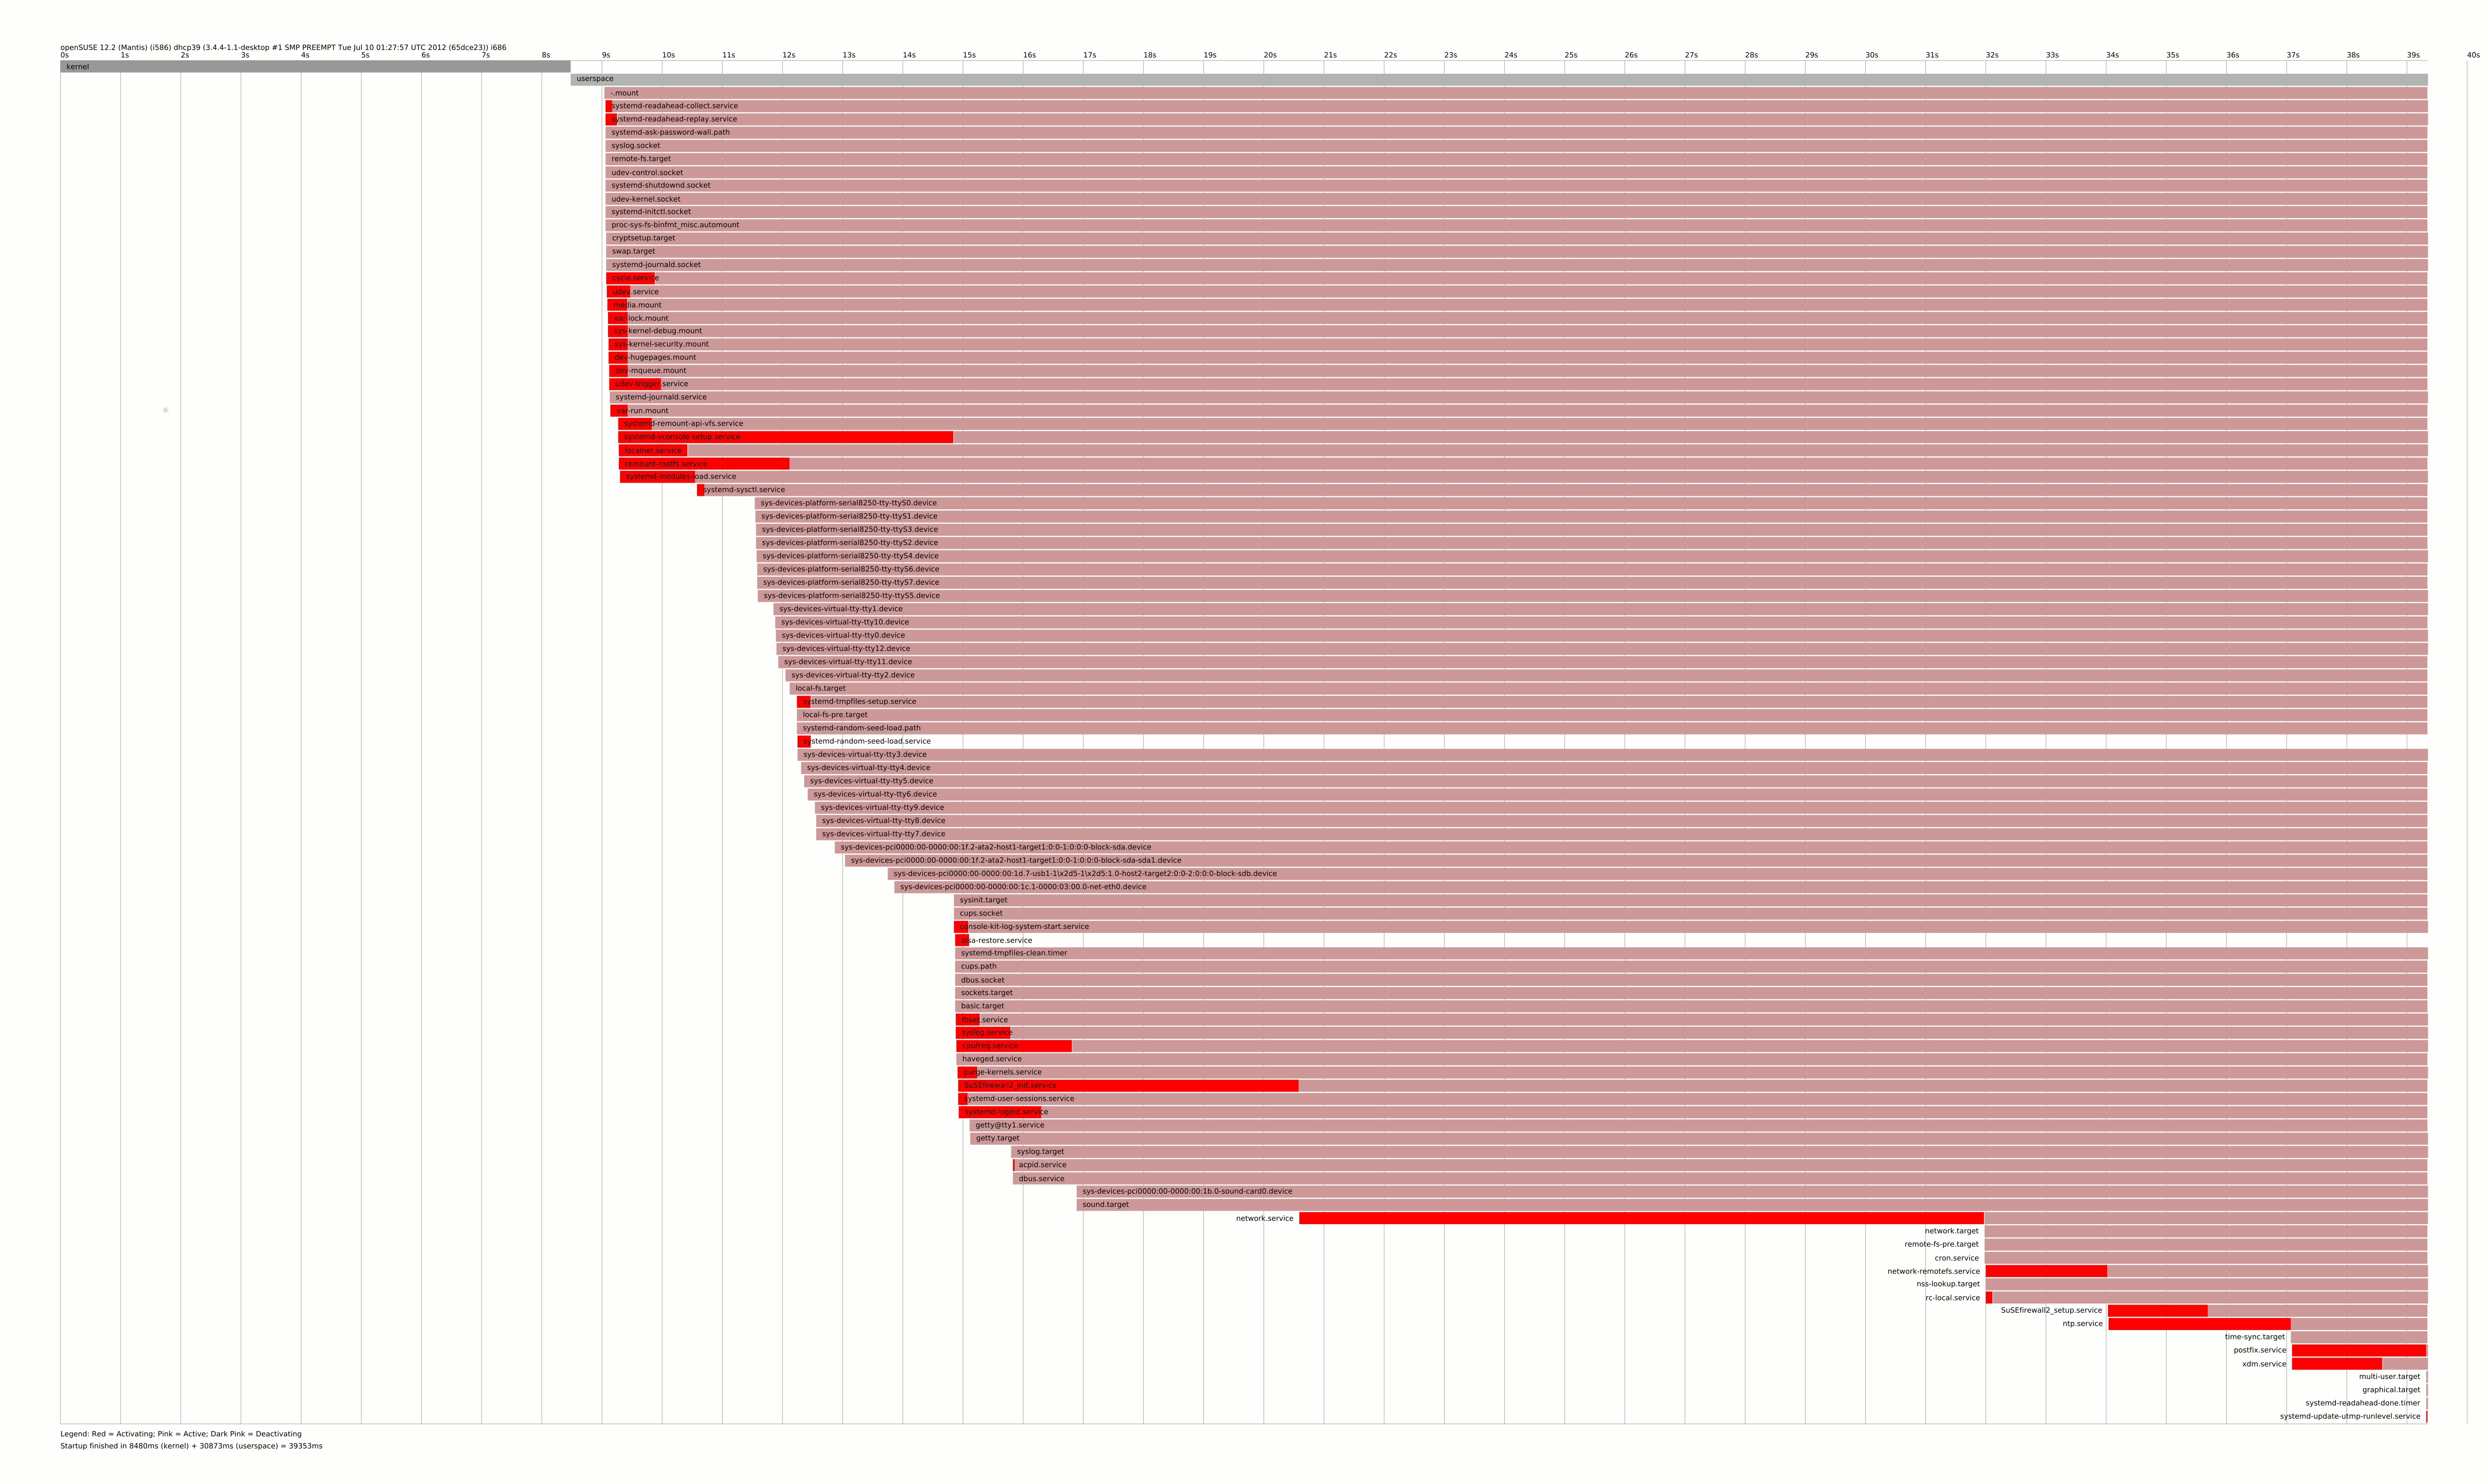
\includegraphics[width=\textwidth]{figs/systemd-analyze-plot.png}
	\begin{itemize}
		\item Similar to bootchartd, but does not require rebooting with a custom \texttt{init=} kernel command-line
	\end{itemize}
\end{frame}

\begin{frame}[fragile]{systemd-analyze critical-chain}
	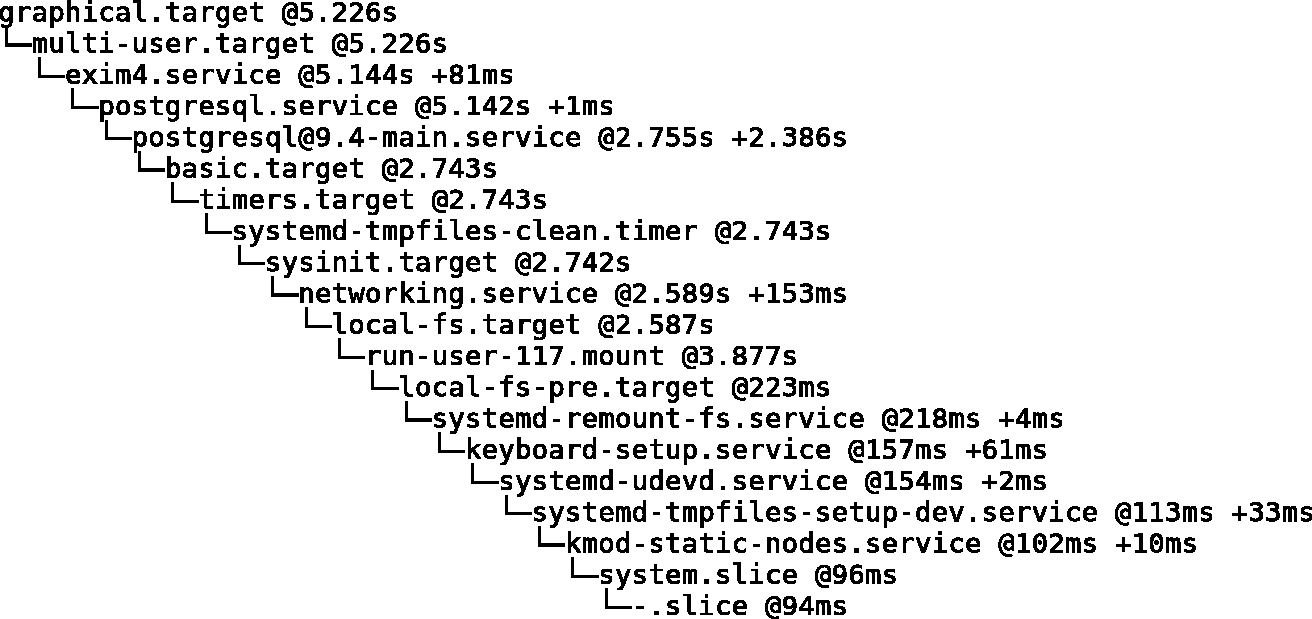
\includegraphics[width=\textwidth]{figs/systemd-analyze-critical-chain.pdf}
\end{frame}

\section{Exploring the system status}

\begin{frame}{Exploring the system status}
\begin{itemize}
\item Listing units with \texttt{systemctl list-units} (or just \texttt{systemctl}):
\begin{itemize}
\item active units: \texttt{systemctl}
\hhbr
\item List only services: \texttt{systemctl -t service}
\hhbr
\item List units in failed state: \texttt{systemctl --failed}
\end{itemize}
\hbr
\item Whole system overview: \texttt{systemctl status}
\hbr
\item GUI available: \texttt{systemadm}
\end{itemize}
\end{frame}

\begin{frame}{\texttt{systemctl status \textsl{\tt service}}}
\br
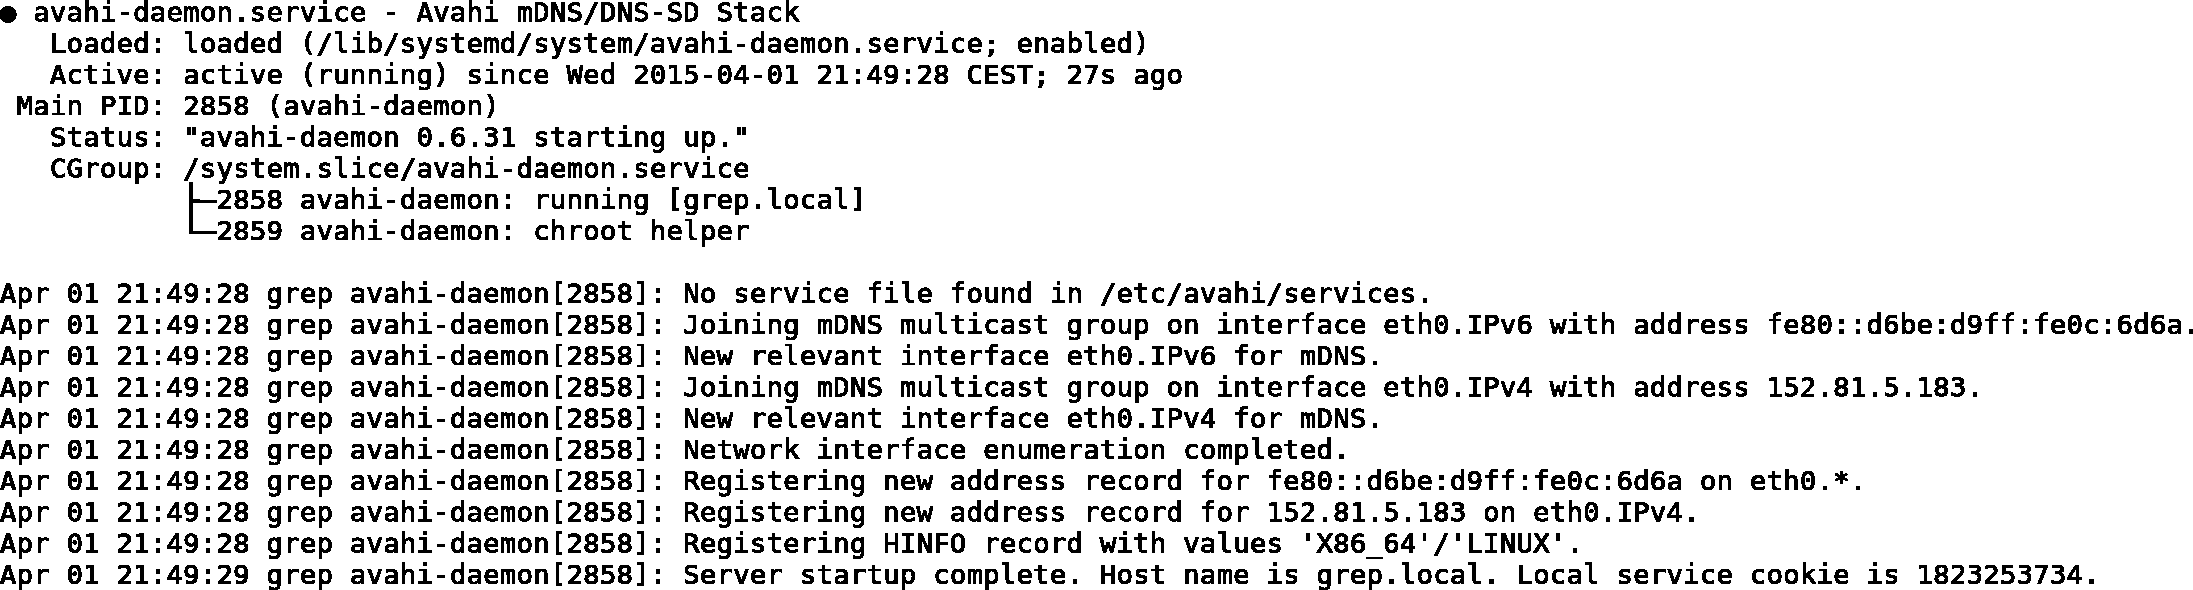
\includegraphics[width=1.5\textwidth]{figs/systemctl-status}
\hbr
Includes:
\begin{itemize}
\item Service name and description, state, PID
\item Free-form status line from \texttt{systemd-notify(1)} or \texttt{sd\_notify(3)}
\item Processes tree inside the cgroup
\item Last lines from journald (syslog messages and stdout/stderr)
\end{itemize}
\end{frame}

\section{Writing unit files}

\begin{frame}{Writing unit files}
\begin{itemize}
\item With sysVinit: shell scripts in \texttt{/etc/init.d/}
\begin{itemize}
\item Long and difficult to write
\item Redundant code between services
\item Slow (numerous forks() calls)
\end{itemize}
\hbr
\item With systemd: declarative syntax (.desktop-like)
\begin{itemize}
\item Most of the intelligence is moved from the script to systemd
\item Covers most of the needs, but shell scripts can still be used
\item Can use includes and overrides (\texttt{systemd-delta})
\item View unit file for a service: \texttt{systemctl cat atd.service}
\item Or just find the file under \texttt{/lib/systemd/system/} (distribution's defaults) or \texttt{/etc/systemd/system} (local overrides)
\end{itemize}
\end{itemize}
\end{frame}

\begin{frame}[fragile]{Simple example: atd}
\begin{lstlisting}[basicstyle=\ttfamily\normalsize,escapeinside={||}]
[Unit]
Description=Deferred execution scheduler
|\alert{\# Pointer to documentation shown in systemctl status}|
Documentation=man:atd(8)

[Service]
|\alert{\# Command to start the service}|
ExecStart=/usr/sbin/atd -f
IgnoreSIGPIPE=false |\alert{\# Default is true}|

[Install]
|\alert{\# Indicates reverse-dependency}|
WantedBy=multi-user.target
\end{lstlisting}
\end{frame}

\begin{frame}[fragile]{Common options}
\hbr
\begin{itemize}
\item Documented in \texttt{systemd.unit(5)} ([Unit]), \texttt{systemd.service(5)} ([Service]), \texttt{systemd.exec(5)} (execution environment)
\hbr
\item Show all options for a given service:\\
\texttt{systemctl show atd}
\hbr
	\item Sourcing a configuration file:\\
\texttt{EnvironmentFile=-/etc/default/ssh}\\
\texttt{ExecStart=/usr/sbin/sshd -D \$SSHD\_OPTS}
\hbr
\item Using the \texttt{\$MAINPID} magic variable:\\
\texttt{ExecReload=/bin/kill -HUP \$MAINPID}
\hbr
\item Auto-restart a service when crashed:\\
\texttt{Restart=on-failure}
\hbr
\item Conditional start:\\
\texttt{ConditionPathExists=!/etc/ssh/sshd\_not\_to\_be\_run}\\
Also conditions on architecture, virtualization, kernel command-line, AC power, path properties, etc.
\end{itemize}
\end{frame}

\begin{frame}{Options for isolation and security}
	\begin{itemize}
		\item Use a network namespace to isolate the service from the network:\\
			\texttt{PrivateNetwork=yes}
			\hbr
		\item Use a filesystem namespaces:
			\begin{itemize}
				\item To provide a service-specific \texttt{/tmp} directory:\\
					\texttt{PrivateTmp=yes}
					\hbr
				\item To make some directories inaccessible or read-only:\\
					\texttt{InaccessibleDirectories=/home}\\
					\texttt{ReadOnlyDirectories=/var}
			\end{itemize}
			\hbr
		\item Specify the list of \texttt{capabilities(7)} for a service:\\
			\texttt{CapabilityBoundingSet=CAP\_CHOWN CAP\_KILL}\\
			Or just remove one:\\
			\texttt{CapabilityBoundingSet=\textasciitilde{}CAP\_SYS\_PTRACE}
			\hbr
		\item Disallow forking:\\
			\texttt{LimitNPROC=1}
	\end{itemize}
\end{frame}
\begin{frame}{Options for isolation and security (2)}
\begin{itemize}
		\item Run as user/group: \texttt{User=}, \texttt{Group=}
			\hbr
		\item Run service inside a chroot:\\
			\texttt{RootDirectory=/srv/chroot/foobar}\\
			\texttt{ExecStartPre=/usr/local/bin/setup-foobar-chroot.sh}\\
			\texttt{ExecStart=/usr/bin/foobard}\\
			\texttt{RootDirectoryStartOnly=yes}
			\hbr
		\item Control CPU shares, memory limits, block I/O, swapiness:\\
			\texttt{CPUShares=1500}\\
			\texttt{MemoryLimit=1G}\\
			\texttt{BlockIOWeight=500}\\
			\texttt{BlockIOReadBandwith=/var/log 5M}\\
			\texttt{ControlGroupAttribute=memory.swappiness 70}
			\hbr
		\item More information:
				\href{http://0pointer.net/blog/projects/systemd-for-admins-3.html}{\ul{Converting sysV init scripts to systemd service files}},
				\href{http://0pointer.net/blog/projects/security.html}{\ul{Securing your services}},
				\href{http://0pointer.net/blog/projects/changing-roots.html}{\ul{Changing roots}},
				\href{http://0pointer.net/blog/projects/resources.html}{\ul{Managing resources}}
	\end{itemize}
\end{frame}

\section{Timer units}

\begin{frame}{Timer units}
	\begin{itemize}
		\item Similar to cron, but with all the power of systemd (dependencies, execution environment configuration, etc)
		\hbr
	\item \alert{Realtime (wallclock) timers}: calendar event expressions
			\begin{itemize}
				\item Expressed using a complex format (see \texttt{systemd.time(7)}), matching timestamps like:
					\texttt{Fri 2012-11-23 11:12:13}
				\hbr
			\item Examples of valid values:  \texttt{hourly} (= \texttt{*-*-* *:00:00}), \texttt{daily} (= \texttt{*-*-* 00:00:00}), \texttt{*:2/3} (= \texttt{*-*-* *:02/3:00})
		\end{itemize}
		\hbr
	\item \alert{Monotonic timers}, relative to different starting points:
		\begin{itemize}
			\item 5 hours and 30 mins after system boot: \texttt{OnBootSec=5h 30m}
				\hbr
			\item 50s after systemd startup: \texttt{OnstartupSec=50s}
				\hbr
			\item 1 hour after the unit was last activated: \texttt{OnUnitActiveSec=1h}\\
				(can be combined with \texttt{OnBootSec} or \texttt{OnStartupSec} to ensure that a unit runs on a regular basis)
		\end{itemize}
	\end{itemize}
\end{frame}

\begin{frame}[fragile]{Timer units example}
\begin{itemize}
\item \texttt{myscript.service}:
\begin{lstlisting}[basicstyle=\ttfamily\footnotesize,escapeinside={||}]
[Unit]
Description=MyScript

[Service]
Type=simple
ExecStart=/usr/local/bin/myscript
\end{lstlisting}
\item \texttt{myscript.timer}:
\begin{lstlisting}[basicstyle=\ttfamily\footnotesize,escapeinside={||}]
[Unit]
Description=Runs myscript every hour

[Timer]
# Time to wait after booting before we run first time
OnBootSec=10min
# Time between running each consecutive time
OnUnitActiveSec=1h
Unit=myscript.service

[Install]
WantedBy=multi-user.target
\end{lstlisting}
\end{itemize}
\end{frame}
\begin{frame}{Timer units example (2)}
	\begin{itemize}
\item Start timer:\\ \texttt{systemctl start myscript.timer}
	\hbr
\item Enable timer to start at boot:\\
	\texttt{systemctl enable myscript.timer}
\hbr
\item List all timers:\\ \texttt{systemctl list-timers}
\end{itemize}
\end{frame}

\section{Socket activation}

\begin{frame}{Socket activation}
\begin{itemize}
\item Similar to inetd:
	\begin{itemize}
		\item The service is not started automatically at boot
		\item systemd listens for connections on behalf of service
		\item systemd starts the service to handle the connection
	\end{itemize}
\hbr
\item Useful for services that are seldomly used: cups, sshd
\hbr
\item Same idea for dbus activation and fs activation (autofs-like)
\hbr
\item Also makes it possible to parallelize startup\\ {\small (synchronization on first interaction using sockets)}
\hbr
\item More information: \href{http://0pointer.net/blog/projects/inetd.html}{\ul{Converting inetd Service}}, \href{http://0pointer.net/blog/projects/socket-activation.html}{\ul{Socket Activation for developers}} (+ \href{http://0pointer.net/blog/projects/socket-activation2.html}{\ul{follow-up}})
\end{itemize}
\end{frame}

\begin{frame}[fragile]{Socket activation example (sshd)}
\begin{itemize}
\item \texttt{sshd.socket}:
\begin{lstlisting}[basicstyle=\ttfamily\footnotesize,escapeinside={||}]
[Unit]
Description=SSH Socket for Per-Connection Servers

[Socket]
ListenStream=22
Accept=yes

[Install]
WantedBy=sockets.target
\end{lstlisting}
\item \texttt{sshd@.service}:
\begin{lstlisting}[basicstyle=\ttfamily\footnotesize,escapeinside={||}]
[Unit]
Description=SSH Per-Connection Server

[Service]
ExecStart=-/usr/sbin/sshd -i
StandardInput=socket
\end{lstlisting}
\end{itemize}
\end{frame}

\begin{frame}[fragile]{Socket activation example (sshd) (2)}
\begin{itemize}
	\item \texttt{sshd@.service} means that this is an \alert{instanciated service}
	\hbr
\item There's one instance of \texttt{sshd@.service} per connection:
\end{itemize}
\begin{lstlisting}[basicstyle=\ttfamily\scriptsize]
# systemctl --full | grep ssh
sshd@172.31.0.52:22-172.31.0.4:47779.service  loaded active running
sshd@172.31.0.52:22-172.31.0.54:52985.service loaded active running
sshd.socket                                   loaded active listening
\end{lstlisting}
\begin{itemize}
\item Instanciated services are also used by getty, for example\\
	See \href{http://0pointer.de/blog/projects/serial-console.html}{\ul{Serial console}}
	and \href{http://0pointer.de/blog/projects/instances.html}{\ul{Instanciated services}}
\end{itemize}
\end{frame}

\section{Logging with journald}

\begin{frame}{Logging with journald}
\begin{itemize}
\item Component of systemd
\hbr
\item Captures syslog messages, kernel log messages, initrd and early boot messages, messages written to stdout/stderr by all services
	\begin{itemize}
		\item Forwards everything to syslog
	\end{itemize}
\hbr
\item Structured format (key/value fields), can contain arbitrary data
\begin{itemize}
\item But viewable as syslog-like format with \texttt{journalctl}
\end{itemize}
\hbr
\item Indexed, binary logs
\hbr
\item Can replace syslog (but can also work in parallel)
\hbr
\item Not persistent across reboots by default -- to make it persistent:\\
	\texttt{mkdir -p /var/log/journal}
\hbr
\item Can log to a remote host (with \texttt{systemd-journal-gateway}, not in Debian yet)
\end{itemize}
\end{frame}

\begin{frame}[fragile]{Example journal entry}
\begin{lstlisting}[basicstyle=\ttfamily\small]
_SERVICE=systemd-logind.service
MESSAGE=User harald logged in
MESSAGE_ID=422bc3d271414bc8bc9570f222f24a9
_EXE=/lib/systemd/systemd-logind
_COMM=systemd-logind
_CMDLINE=/lib/systemd/systemd-logind
_PID=4711
_UID=0
_GID=0
_SYSTEMD_CGROUP=/system/systemd-logind.service
_CGROUPS=cpu:/system/systemd-logind.service
PRIORITY=6
_BOOT_ID=422bc3d271414bc8bc95870f222f24a9
_MACHINE_ID=c686f3b205dd48e0b43ceb6eda479721
_HOSTNAME=waldi
LOGIN_USER=500
\end{lstlisting}
\end{frame}

\begin{frame}{Using \texttt{journalctl}}
	\begin{itemize}
		\item View the full log: \texttt{journalctl}
			\hbr
		\item Since last boot: \texttt{journalctl -b}
			\hbr
	\item For a given time interval: \texttt{journalctl --since=yesterday}\\
		or \texttt{journalctl --until="2013-03-15 13:10:30"}
			\hbr
		\item View it in the verbose (native) format: \texttt{journal -o verbose}
			\hbr
		\item Filter by systemd unit: \texttt{journalctl -u ssh}
			\hbr
		\item Filter by field from the verbose format:\\
			\texttt{journalctl \_SYSTEMD\_UNIT=ssh.service}\\
			\texttt{journalctl \_PID=810}
			\hbr
		\item Line view ($\approx$ tail -f): \texttt{journalctl -f}
			\hbr
		\item Last entries ($\approx$ tail): \texttt{journalctl -n}
		\hbr
		\item Works with bash-completion (beware of sudo though)
			\hbr
		\item See also: \href{https://docs.google.com/document/pub?id=1IC9yOXj7j6cdLLxWEBAGRL6wl97tFxgjLUEHIX3MSTs}{\ul{Journald design document}}, \href{http://0pointer.net/blog/projects/journalctl.html}{\ul{Using the Journal}}

	\end{itemize}
\end{frame}

\begin{frame}{Containers integration}
\begin{itemize}
	\item General philosophy: \alert{integrate management of services from machines (VMs and containers) with those of the host}
	\begin{itemize}
		\item \texttt{systemd-machined}: tracks machines, provides an API to list, create, register, kill, terminate machines
			\hbr
		\item \texttt{machinectl}: command-line utility to manipulate machines
			\hbr
		\item other tools also have containers support:
			\begin{itemize}
				\item \texttt{systemctl -M mycontainer restart foo}
				\item \texttt{systemctl list-machines}: provides state of containers
				\item \texttt{journalctl -M mycontainer}
				\item \texttt{journalctl -m}: combined log of all containers
			\end{itemize}
	\end{itemize}
\hbr
\item systemd has its own mini-container manager: \texttt{systemd-nspawn}
\hbr
\item Other virtualization solutions can also \href{http://www.freedesktop.org/wiki/Software/systemd/machined/}{\ul{talk to \texttt{machined}}}
\hbr
\item More information: \href{http://0pointer.net/blog/systemd-for-administrators-part-xxi.html}{\ul{Container integration}}
\end{itemize}
\end{frame}

\begin{frame}{From the service developer's point of view}
	\begin{itemize}
		\item Much easier to write service files than sysVinit scripts
			\hbr
		\item Many things can be handled by systemd for free:
			\begin{itemize}
				\item No need to fork
					\hbr
				\item No need to drop privileges
					\hbr
				\item No need to write a pid file
					\hbr
				\item Can just output logs to stdout (with systemd, stdout will go to journald and syslog)
					\begin{itemize}
						\item \href{http://0pointer.net/blog/projects/journal-submit.html}{\ul{Priorities are even supported}}
					\end{itemize}
			\end{itemize}
	\end{itemize}
\end{frame}

\begin{frame}{More stuff}
	\begin{itemize}
		\item \href{http://0pointer.net/blog/projects/the-new-configuration-files.html}{\ul{New cross-distro configuration files}}: \texttt{/etc/hostname}, \texttt{/etc/locale.conf}, \texttt{/etc/sysctl.d/*.conf}, \texttt{/etc/tmpfiles.d/*.conf}
			\hbr
		\item \href{http://www.certdepot.net/rhel7-get-started-systemd/}{\ul{Tools to manage hostname, locale, time and date}}: \texttt{hostnamectl}, \texttt{localectl}, \texttt{timedatectl}
			\hbr
		\item \href{http://0pointer.net/blog/projects/watchdog.html}{\ul{Support for watchdogs}}
			\hbr
		\item Handling of user sessions
			\begin{itemize}
				\item Each within its own cgroup
					\hbr
				\item \href{http://0pointer.net/blog/projects/multi-seat.html}{\ul{Multi-seat support}}
					\hbr
				\item \texttt{loginctl} to manage sessions, users, seats
			\end{itemize}
			\hbr
		\item systemd networking: systemd-networkd, systemd-resolved
	\end{itemize}
\end{frame}

\end{document}
